\documentclass[tikz,border=5pt]{standalone}
\usepackage{luatexja}
\usepackage[hiragino-pron]{luatexja-preset}
\usepackage{amsmath,amssymb}
\usetikzlibrary{arrows.meta,patterns}

\begin{document}
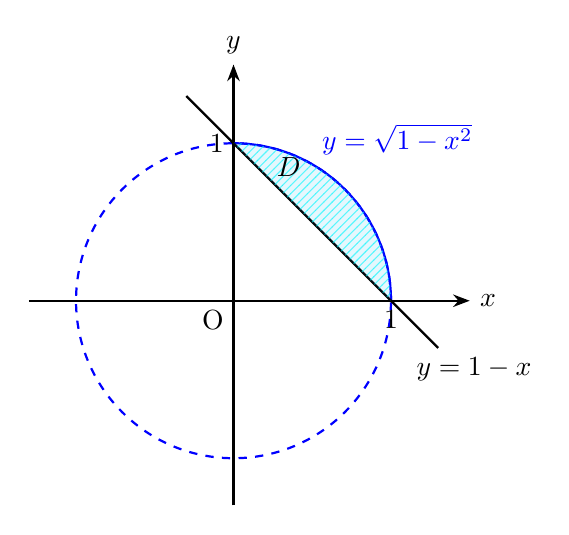
\begin{tikzpicture}[scale=2]

% Axes
\draw[-{Stealth[length=6pt]}, thick] (-1.3,0) -- (1.5,0) node[right] {$x$};
\draw[-{Stealth[length=6pt]}, thick] (0,-1.3) -- (0,1.5) node[above] {$y$};

% Unit circle
\draw[thick, blue, dashed] (0,0) circle (1);
\draw[thick, blue] (1,0) arc[start angle=0, end angle=90, radius=1];

% Line x + y = 1
\draw[thick, black, domain=-0.3:1.3, samples=2] plot (\x, {1-\x});

% Fill region D (inside circle, above line x+y=1)
\fill[pattern=north east lines, pattern color=cyan, opacity=0.6]
  plot[domain=0:1, samples=60, smooth] (\x, {sqrt(1-\x*\x)})
  -- plot[domain=1:0, samples=2] (\x, {1-\x})
  -- cycle;
\fill[cyan, opacity=0.1]
  plot[domain=0:1, samples=60, smooth] (\x, {sqrt(1-\x*\x)})
  -- plot[domain=1:0, samples=2] (\x, {1-\x})
  -- cycle;

% Labels
\node[below left] at (0,0) {O};
\node[below] at (1,0) {$1$};
\node[left] at (0,1) {$1$};
\node[below right, black] at (1.1,-0.3) {$y = 1 - x$};
\node[above right, blue] at (0.5,{sqrt(1-0.25)}) {$y = \sqrt{1-x^2}$};
\node at (0.35,0.85) {$D$};

% y = sqrt(1-x^2) label
\node[above right] at (0.6, {sqrt(1-0.36)}) {};

\end{tikzpicture}
\end{document}
